\section{Forsøg 1 - Kredsløb}

\subsection{Forsøgsbeskrivelse}

\subsubsection{Formål}
Formålet med disse forsøg er at for en forståelse af, hvordan de forskellige kredsløb fungere. Derudover bliver der også dannet en baggrundsviden af, hvordan det teoretiske er i kredsløbet. Måledataenes vær-dier kan senere bruges til, at beregne på de forskellige komponenter i kredsløbet. Ud fra måledataene kan der findes en induktans på spolen, som senere kan benyttes til værdi i Plecs, så vores forsøg beskrivelser også kan simuleres, derudover benyttes måledataene også til, at regne på andre forskellige komponenter. Alt dette findes i afsnittet med beregninger. Formlerne som bliver benyttet igennem dette afsnit, til at beregne på forsøget, er alle fundet i kilden \cite{fysikbog}.

\subsubsection{LC serie kredsløb}
%\textbf{LC Serie kredsløb}

Komponenter:

\begin{itemize}
\item Generator $(50\, \Omega$ modstand)
\item Kapacitor $( 0,1\, \mu F)$
\item Spole/Inductor $(1600$ vindinger)
\item Oscilloskop
\end{itemize}

Opstilling:

\begin{figure}[H]
\centering
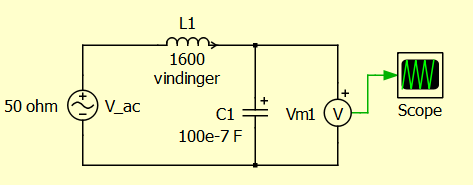
\includegraphics[scale=1]{Vildledning/Schematics/Kredslb/LC_Serie}
\caption{LC Serie Kredsløb}
\label{lcserie}
\end{figure}

Figur \ref{lcserie} viser, hvordan forsøgsopstillingen er bygget op. Forsøget består af en generator, spole og en kapacitor, hvor der sat et oscilloskop til.

\subsubsection{LC parallel kredsløb}

Komponenter:

\begin{itemize}
\item Generator $(600\, \Omega$ modstand)
\item Kapacitor $( 0,1\, \mu F)$
\item Spole/Inductor $(1600$ vindinger)
\item Oscilloskop
\end{itemize}

Opstilling:

\begin{figure}[H]
\centering
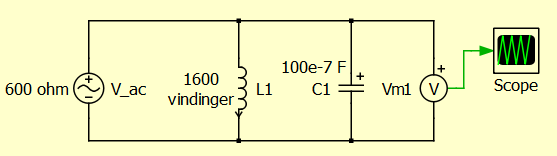
\includegraphics[scale=1]{Vildledning/Schematics/Kredslb/LC_Parallel}
\caption{LC Parallel Kredsløb}
\label{lcparallel}
\end{figure}

Figur \ref{lcparallel} viser forsøgsopstilling af et LC parallel kredsløb, hvor hele kredsløbet sidder parallelt. Kredsløbet er bestående af en generator, en spole og en kapacitor, hvor et oscilloskop er sat til.

\subsubsection{LCR målt over spolen}

Komponenter:

\begin{itemize}
\item Generator $(50\, \Omega$ modstand)
\item Kapacitor $( 0,1\, \mu F)$
\item Spole/Inductor $(1600$ vindinger)
\item Modstand/Resistance $(500\, \Omega)$
\item Oscilloskop
\end{itemize}

Opstilling:

\begin{figure}[H]
\centering
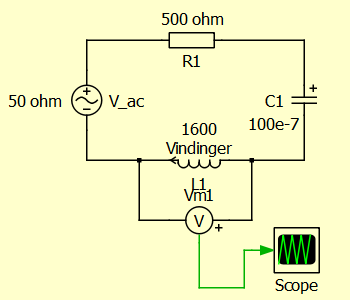
\includegraphics[scale=1]{Vildledning/Schematics/Kredslb/LCR_spole}
\caption{LCR-kredsløb målt over spolen}
\label{figure:lcrspole}
\end{figure}

Figur \ref{figure:lcrspole} viser forsøgsopstilling af et LCR-kredsløb. I dette forsøg bliver der målt over spolen, altså oscilloskopet er sat over spolen. Kredsløbet består af en generator, en spole, en kapacitor og en modstand.

\subsubsection{LCR målt over modstand}

Komponenter:

\begin{itemize}
\item Generator $(50\, \Omega$ modstand)
\item Kapacitor $( 0,1\, \mu F)$
\item Spole/Inductor $(1600$ vindinger)
\item Modstand/Resistance $(500\, \Omega)$
\item Oscilloskop
\end{itemize}


Opstilling:

\begin{figure}[H]
\centering
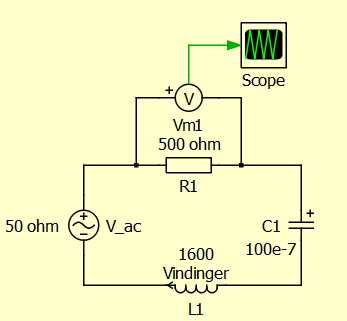
\includegraphics[scale=1]{Vildledning/Schematics/Kredslb/LCR_modstand}
\caption{LCR-kredsløb målt over spolen}
\label{lcrmodstand}
\end{figure}

Figur \ref{lcrmodstand} viser forsøgsopstilling af et LCR-kredsløb. Modsat tidligere forsøg, så bliver der målt over modstanden. Kredsløbet er bestående af samme komponenter som det tidligere forsøg.

\subsection{Fremgangsmåde}

Udførelsen af forsøgende er næsten ens, de variere ikke ret meget, forsøgsopstillingen bliver ændret fra forsøgs til forsøg, hvor der skiftets ud i komponenter, så det passer med det rigtige kredsløb.

Først opstilles kredsløbet, som det er vist på figurene \ref{lcserie}, \ref{lcparallel}, \ref{figure:lcrspole} og \ref{lcrmodstand}. Derefter skal oscilloskopet indstilles, så det måler de rigtige data, det indstilles til at måle en: peak-to-peak. Så er forsøget klar til at starte, der tændes for generatoren, og dens frekvens indstilles til den ønskede værdi, og peak-to-peak værdien noteres. Dette gøres med forskellige frekvenser, så der fås forskellige data, som senere kan plottes ind i en tabel, og der kan derved laves en graf for det.

\subsection{Resultater}

LC-kredsløb (Kapacitor):

For LC-kredsløbet blev der foretaget målinger for spændingen over kapacitoren ved forskellige frekvenser. Første måling er foretaget ved $1 \, kHz$, hvorefter de følgende målinger er foretaget med et $0,5\, kHz$ interval op til sidste måling ved $5,5\, kHz$. Resultaterne er indsat i nedenstående graf. Tabel \ref{tabular:lcserie} angiver resultaterne for spændingen i forhold til den givne frekvens.

\begin{figure}[H]
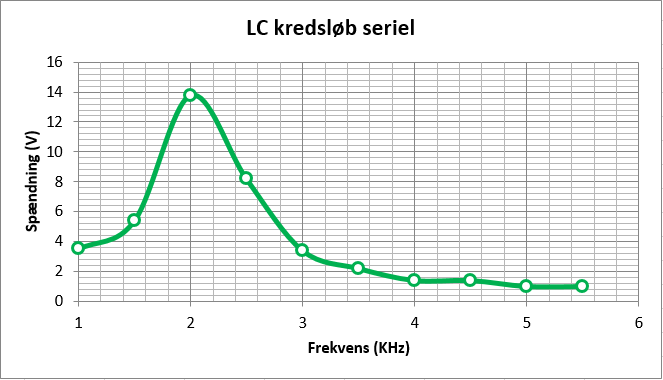
\includegraphics[scale=1]{Setup/Graf3}
\caption{}
\label{graph:lcserie}
\end{figure}

\begin{table}[H]
\centering
\begin{tabular}{|r|r|r|r|r|r|r|r|r|r|r|} \hline
kHz & 1 & 1,5 & 2 & 2,5 & 3 & 3,5 & 4 & 4,5 & 5 & 5,5 \\ \hline
V & 3,5 & 5,4 & 13,8 & 8,2 & 3,4 & 2,2 & 1,4 & 1,4 & 1 & 1 \\ \hline
\end{tabular}
\caption{}
\label{tabular:lcserie}
\end{table}

Graf \ref{graph:lcserie} viser sammenhængen mellem spændingen og frekvensen over kapacitoren, når frekvensen øges. Ved en frekvens på $1\, kHz$ er spændingen over kapacitoren $3,5\, V$. Ved en frekvens på $1,5\, kHz$ er spændingen øget til $5,4\, V$, hvorefter der sker en markant stigning til en spænding på $13,8\, V$ ved en frekvens på $2\, kHz$. Fra frekvensen på $2 kHz$ og til en frekvens på $4\, kHz$ er spændingen over kapacitoren faldet til $1,4\, V$, hvorefter funktionen flader ud, og spændingen næsten holdes stabil til en frekvens på $5,5\, kHz$.

LCR-kredsløb (Resistor):

Første sæt målinger for LCR-kredsløbet angiver spændingen over resistoren ved en stigende frekvens. Målingerne er foretaget fra $1\, kHz$ til $10\, kHz$ med et interval på $1\, kHz$ for hver måling. Resultaterne for målingerne er plottet i nedenstående graf. Tabel \ref{tabular:lcrmodstand} angiver resultaterne for spændingen i forhold til den givne frekvens.

\begin{figure}[H]
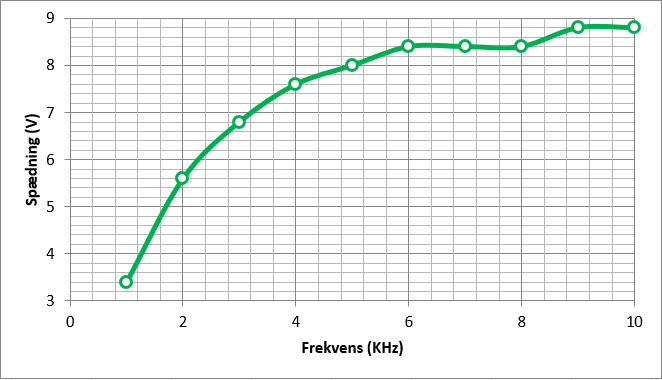
\includegraphics[scale=1]{Setup/Graf7}
\caption{}
\label{graph:lcrmodstand}
\end{figure}

\begin{table}[H]
\centering
\begin{tabular}{|r|r|r|r|r|r|r|r|r|r|r|} \hline
kHz & 1 & 2 & 3 & 4 & 5 & 6 & 7 & 8 & 9 & 10 \\ \hline
V & 3,4 & 5,6 & 6,8 & 7,6 & 8 & 8,4 & 8,4 & 8,4 & 8,8 & 8,8 \\ \hline
\end{tabular}
\caption{}
\label{tabular:lcrmodstand}
\end{table}

Graf \ref{graph:lcrmodstand} viser, hvordan spændingen over resistoren er lav ved en frekvens på $1\, kHz$. Ved en stigning i frekvens viser det sig, at spændingen stiger som en eksponentielt aftagende funktion. Fra en frekvens på $1\, kHz$ til $4\, kHz$ stiger spændingen over modstanden fra $3,4\, V$ til $7,6\, V$, men ved de efterfølgende stigninger i frekvens flader funktionen ud, og der sker kun en spændingsstigning på $0,4\, V$ fra en frekvens på $6\, kHz$ til $10\, kHz$.

LCR-kredsløb (Spole):

De næste målinger der er foretaget på LCR-kredsløbet viser sammenhængen mellem spændingen og frekvensen for induktoren. Her foretages målingerne igen ved en frekvens fra $1\, kHz$ til $10\, kHz$ med et stigende interval på $1\, kHz$. Nedenstående graf viser resultaterne for forsøget, hvor tabel \ref{tabular:lcrspole} angiver resultaterne for spændingen i forhold til den givne frekvens.

\begin{figure}[H]
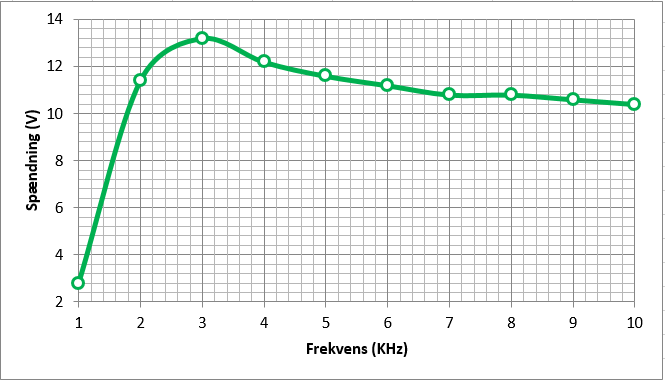
\includegraphics[scale=1]{Setup/Graf6}
\caption{}
\label{graph:lcrspole}
\end{figure}

\begin{table}[H]
\centering
\begin{tabular}{|r|r|r|r|r|r|r|r|r|r|r|} \hline
kHz & 1 & 2 & 3 & 4 & 5 & 6 & 7 & 8 & 9 & 10 \\ \hline
V & 2,8 & 11,4 & 13,2 & 12,2 & 11,6 & 11,2 & 10,8 & 10,8 & 10,6 & 10,4 \\ \hline
\end{tabular}
\caption{}
\label{tabular:lcrspole}
\end{table}

Spændingen over induktoren stiger fra $2,8\, V$ ved en frekvens på $1\, kHz$ til $11,4\, V$ ved en frekvens på $2\, kHz$. Spændingen stiger fortsat til $13,2\, V$ ved en frekvens på $3\, kHz$, hvorefter spændingen over induktoren begynder at falder ved en højere frekvens. Faldet i spændingen sker kun gradvist og ved en frekvens på $7\, kHz$, er funktionen næsten ved en stabil spænding.

\subsection{Databehandling}

%\subsubsection{"LC kredsløb"}

\begin{equation} \label{angfreq}
\omega = \frac{1}{\sqrt{LC}}
\end{equation}

Denne ligning for vinkelbestemt frekvens relaterer: frekvens, kapacitans og induktans.

Der løses for L da denne er besværlig at måle sammenlignet med den aflæste kapacitans. $\omega = 2\pi f$ så denne indsættes samtidigt:

\begin{equation}
\omega = \frac{1}{\sqrt{LC}} \Leftrightarrow L = \frac{1}{\omega^2 \cdot C} = \frac{1}{4\pi^2 f^2 \cdot C} = \frac{1}{4\cdot \pi^2 f^2\cdot 0.1\mu F}
\end{equation}


\subsubsection{LCR kredsløb}

\begin{table}[H]
\centering
\begin{tabular}{l|l}
Induktans  & 0,0525 $H$ \\ 
Kapacitans & 0.1 $\mu F$   \\
Amplitude  & 10,0 $V$   \\
Modstand   & 500 $\Omega$ \\
\end{tabular}
\caption{Værdier for komponenter}
\label{tabular:value}
\end{table}

I afsnit 4.2 blev der redegjort for resonant frekvens. Der blev nævnt at ved resonant frekvens, at strømmen gennem spolen og kapacitansen fuldstændig udeligner hinanden, altså strømmen gennem dem giver $0$.

Forsøget med LCR-kredsløbet afbillede, hvordan spændingen er afhængig af hvilken frekvens, der benyttes. Samtidig svinger den samlede impedans i kredsløbet og ud fra det, kan strømmen beregnes for kredsløbet. Ud fra dette viser det sig, at strømstyrken også varierer i forhold til frekvensen, hvor strømmen når maksimum ved systemets resonante frekvens. Her er modstanden afgørende for, hvordan strømstyrken opfører sig ved forskellige frekvenser. Ved en lav modstand i systemet vil strømstyrken ved den resonante frekvens være meget høj i forhold til andre frekvenser, mens en stor modstand vil mindske udslaget. Til gengæld vil en stor modstand forstørre frekvensområdet, som strømstyrken vil toppe ved.

\begin{figure}[H]
\centering
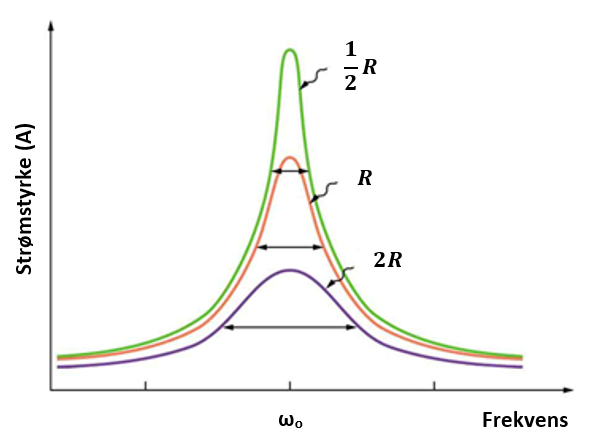
\includegraphics[scale=0.75]{Vildledning/Schematics/Resonanskurver}
\caption{Resonant frekvens ved 3 forskellige modstande \cite{Bresonant}.}
\label{figure:resonantfrekvens}
\end{figure}

Graf \ref{figure:resonantfrekvens} viser tre forskellige grafer over strømstyrken for systemet i forhols til frekvensen. Forskellen på de tre funktioner er, at der er forskellige størrelse modstande til de tre kredsløb. Den grønne graf har en modstand på $\frac{1}{2} R$, hvor strømstyrken giver et stort udsving ved den resonante frekvens. Til gengæld er udsvinget meget smalt, så frekvensen skal ikke afvige meget fra den resonante frekvens, før strømstyrken falder kraftigt. Ved den orange funktion er modstanden i systemet fordoblet. Her foretager strømstyrken igen et stort udsving ved den resonante frekvens, men stadig mindre end den grønne funktion. Til gengæld er udsvinget fladet mere ud, hvorved der kan ske større afvigelser fra den resonante frekvens, uden strømstyrken falder meget. For den lilla funktion, hvor modstanden er på $2 R$, så er udsvinget for strømstyrken lav ved den resonante frekvens i forhold til de to andre funktioner. Derimod strækker grafens udsving sig over et stort frekvensområde.

Grafen viser, at den resonante frekvens vil være optimal for det største output. Herefter afbilleder funktionerne, at den samlede modstand for systemet er afgørende for, hvor stort et output systemet har, og hvor let det er at ramme et højt output. Hvis der skal benyttes en lav strømstyrke, vil det være optimalt at benytte en stor modstand i kredsløbet for at give et bredt frekvensspektrum til den ønskede strøm. Derimod kræver høje output, at modstanden er lavt, hvorved der opstår et stort udslag, men så skal der omhyggeligt korrigeres for den resonante frekvens.

Resonant frekvens er givet ved:

\begin{equation} 
\omega_0 = \frac{1}{\sqrt{LC}}
\label{eq:resonant}
\end{equation}

Med $\omega_0 = 2 \pi f$, dvs. at $\omega_0$ er lig med en fuld svingning $(2\pi)$ ganget med frekvensen $(f)$. Så kan ligning \ref{eq:resonant} løses for frekvensen $f$.

\begin{equation} 
\omega_0 = \frac{1}{\sqrt{LC}} \Leftrightarrow f = \frac{1}{2 \cdot \sqrt{C \cdot L} \cdot \pi}
\label{eq:resonantfrekvens}
\end{equation}

Værdierne fra tabel \ref{tabular:value} benyttes i formlen \ref{eq:resonantfrekvens}, og så findes den resonante frekvens for LCR-kredsløbet.

\begin{equation*}
f = \frac{1}{2 \cdot \pi \cdot \sqrt{(0,1 \cdot 10^-6 F) \cdot 0,0525 H}} = \underline{2197 \, Hz}
\end{equation*}

I afsnit 4.1 og (Impedans afsnit) er der blevet redegjort for formlen for Impedans, den bliver defineret som, $Z$, hvor $Z = R + (X_L - X_C)$. $X_L$ og $X_C$ er blevet nævnt i \vref{eq:kapacitivreaktans} og\vref{eq:induktivreaktans}. Formlen for Impedans bruges også i formlen for at finde peak på strøm igennem kredsløbet. Formlen for strøm peak er:

\begin{equation} 
I_p = \frac{V_p}{\sqrt{R^2 + (X_L - X_C )^2}} = \frac{V_p}{Z}
\label{eq:peak}
\end{equation}

Hvor $V_p$ er volt peak for kredsløbet, denne findes ved: $V_p = \sqrt{V^2_{Rp} + (V_{Lp} - V_{Cp})^2}$, og Impedansen er givet ved $Z = \sqrt{R^2 + (X_L - X_C)^2}$. Så kan de kendte værdier indsættes, og der kan opstilles en graf for $I_p$ og frekvens $f$. Alle data findes i Bilag B (Label til bilag b). Der laves udregninger for en frekvens på $2000 \, Hz$.

$2000 \, Hz$:

$V_p$, $X_L$ og $X_C$ beregnes ud fra formlerne nævnt tidligere.

\begin{equation*}
X_L = 2\pi \cdot 2000 \, Hz \, \cdot 0.0525 \, Hz \, = 659,734 \Omega
\end{equation*}

\begin{equation*}
X_C = \frac{1}{2\pi \cdot 2000 \, Hz \, \cdot (0.1 \cdot 10^{-6} \, F)} = 795,775 \Omega
\end{equation*}

\begin{equation*}
V_p = \sqrt{(9,3 \, V)^2 + (12,3 \, V - 14,8 \, V)^2} = 9,63 V
\end{equation*}

Så kan strøm-peak $I_p$ beregnes:

\begin{equation*}
I_p = \frac{9,63 \, Hz}{\sqrt{(500 \Omega)^2 + (659,734\Omega-795,775\Omega)^2}} = 0,01858 A \cdot 1000 = \underline{18,58 \, mA}
\end{equation*}

Derved er strøm-peak udregnet med en frekvens på $2000 \, Hz$. Denne fremgangsmåde benyttes til at udregne for alle frekvenser, altså fra $1000 \, Hz$ til $10000 \, Hz$, disse data findes i Bilag B (Label dertil). Datasættene er ikke resultaterne fra forsøgene, men de er aflæst efter simulationer af kredsløbet opsat i Plecs. Simulationerne har samme værdier for komponenterne, som komponenterne benyttet i forsøgsopstillingerne.

Ud fra målingerne over LCR-kredsløbet kan strømstyrken for systemet beregnes ud fra en given frekvens, som foretaget tidligere. Herefter kan beregningerne verificeres ved at holdes op mod angivne data fra en simulation af samme kredsløb.

Resultaterne fra simulationen kan også benyttes til at vise udviklingen for strømstyrken ved ændring af frekvensen. Derudover kan der ændres på størrelsen for modstanden på resistoren i systemet for at se, hvordan strømstyrken ændre sit udsving omkring den resonante frekvens.

\begin{figure}[H]
\centering
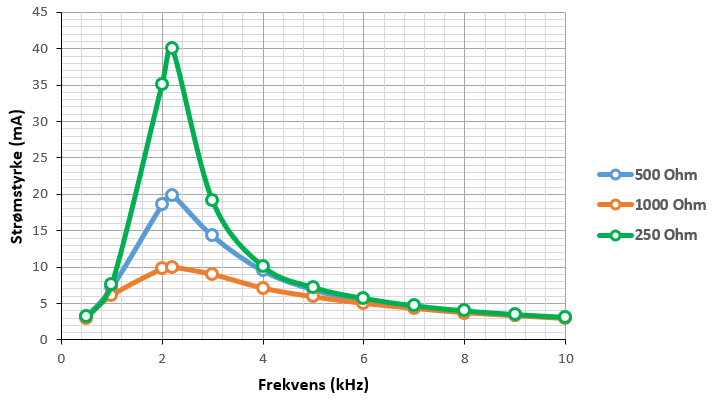
\includegraphics[scale=0.75]{Vildledning/Schematics/Graf_forsg1}
\caption{}
\label{figure:forsg1}
\end{figure}

Graf \ref{figure:forsg1} viser tre funktioner for strømstyrken ved en stigende frekvens. Forskellen på de tre sæt data for funktionerne er, at de henholdsvis har indsat en modstand på $250 \Omega$, $500 \Omega$ eller $1000 \Omega$. Funktionen med modstanden på $250 \Omega$ giver et stort udslag i løbet af en stigning i frekvens mellem $1 kHz$ og $2 kHz$. Toppunktet for funktionen er skarpt optegnet ved den resonante frekvens, hvorefter strømstyrken er blevet mere end halveret ved en frekvens på $3 kHz$. På højere frekvenser falder strømstyrken fortsat, men faldet stilner roligt af. Ved funktionen med en modstand på $500 \Omega$ er udsvinget for strømstyrken ved den resonante frekvens halveret i forhold til første funktion. Til gengæld sker faldet ved større frekvenser ikke så drastisk. Derved bliver frekvensspektret forstørret for et fornuftigt strømstyrkeoutput. Ved den sidste funktion med en modstand på $1000 \Omega$ er udslaget ved den resonante frekvens næste jævnet ud sammenlignet med de to andre funktion. Til gengæld er faldet for strømstyrken lille, og frekvensområdet for en stabil strømstyrke er forlænget meget i forhold til de første to funktioner. Sammenlignet med første funktion, så er det overordnede fald i strømstyrken lav for tredje graf. Hvor den første graf med en modstand på $250 \Omega$ falder med op til 75 procent fra den resonante frekvens på $2.197 kHz$ til $4 kHz$, så sker der kun et fald på 30 procent for den tredje funktion med en modstand på $1000 \Omega$ over samme frekvensområde.

\subsubsection{Beregning af den elektromotoriske spænding}

Ved induktiv kobling er det muligt at beregne den inducerede elektromotoriske spnæding ved hjælp af den magnetiske flux. Ifølge Faraday's lov er den elektromotoriske spænding beskrevet som det negative differentiale af den magnetiske flux i forhold til tiden.

Den benyttede induktor i forsøget er en cylinderformet spole. Det magnetiske felt for spolen er angivet som $\mu_o \cdot n \cdot I$, hvor n er antal vindinger for spolen, og I er strømstyrken. For at beregne den samlede magnetiske flux dannet i spolen, så skal arealet for den cylinderformede spoles tværsnit og længden for spolen ganges på. Tværsnitsarealet for spolen kan opskrives som $2 \pi r^2$, så den magnetiske flux kan beregnes ved $\Phi_B = \mu_o \cdot n \cdot I \cdot 2 \cdot \pi \cdot r^2 \cdot l$. Induktansen for spolen beregnes ved $\mu_o \cdot n \cdot 2 \cdot \pi \cdot r^2$, hvilket kun består af konstanter, så den magnetiske flux kan beskrives som $\Phi_B = L \cdot I$.

Den elektromotoriske spænding for spolen kan nu beskrives ved Faraday's lov:

\begin{equation}
\xi = - \frac{d\Phi_B}{dt}
\end{equation}

Herved kan udtrykket for den magnetiske flux indsættes, så den elektromotoriske spænding kan beregnes ved:

\begin{equation}
\xi = - L \cdot \frac{dI}{dt}
\end{equation}

Faraday's lov beskrives her, hvordan størrelsen på den elektromotoriske spænding er afhængig af en varierende strømstyrke. Strømstyrken kan beskrives ved $I_o \cdot sin(\omega \cdot t + \varphi$, hvor $I_o$ er amplituden for sinusfunktionen, omega er $2 \cdot \pi \cdot f$ og $varphi$ angiver faseforskydelsen for funktionen.

Ved forsøget med LCR-kredsløbet, hvor der foretages målinger over spolen, er det største udslag for spændingen ved $3 kHz$ med en spænding på $13,2 V$. Ved systemet er der indsat en modstand på $500 \Omega$, så amplituden kan beregnes ved $I_o = \frac{U}{R} = \frac{13,2 V}{500 \Omega} = 26,4 mA$. Strømstyrken kan herefter beskrives som en funktion af tiden ved:

\begin{equation}
I = 26,4 mA \cdot sin(2 \pi \cdot 3 kHz \cdot t + \varphi)
\end{equation}

Faseforskydelsen $\varphi$ varierer mellem 0 og $\frac{\phi}{2}$. Hvis forkydelsen er 0, følger funktionen for strømstyrken og spændingen hinanden. Hvis faseforskydelsen er på $\frac{\phi}{2}$, vil funktionen følge en cosinus i stedet.

Herfra kan udtrykket for strømstyrken indsættes i formlen for den elektromotoriske spænding, som derved bliver:

\begin{equation}
\begin{aligned}
&\xi = - L \cdot \frac{dI}{dt} = - 42,3 mH \cdot 26,4 mA \cdot cos(2 \pi \cdot 3 kHz \cdot t +\varphi) \cdot 2 \pi \cdot 3 kHz \\
&= cos(18,85 kHz \cdot t + \varphi) \cdot 21,05 H \cdot A \cdot Hz
\end{aligned}
\end{equation}

Da der ingen tid $(t)$ er, så kan denne ikke beregnes. Ved en kendt tid er det muligt at beregne den elektromotoriske spænding ved modtagerspolen. Beregningen tager udgangspunkt i at finde den overførte energi fra transmitteren til modtageren. Faraday's lov kan benyttes til at beregne det teoretiske udbytte af elektromotorisk spænding ved modtageren ved omdannelse af den magnetiske flux afsendt fra transmitteren. Det skal dog siges, at beregningerne går ud fra, at hele magnetfeltet fra transmitteren når ud til modtageren, så intet går tabt til omgivelserne i luften. Derfor skal resultatet for den elektromotoriske spænding ganges med nyttivirkningen (Se forsøg 2).

Ud fra forsøgende med LCR-kredsløb kom der forskellige værdier for strømstyrken, hvor der tydeligt sker ændringer, afhængig af frekvensen. Ved den resonante frekvens $(2197 \, Hz)$ sker der en stor ændring i strøm, hvor den når helt op på $20,00 \, mA$, hvor den på mindre frekvenser er væsentligt lavere. Ved højere værdier på modstanden sker der også en ændring i værdien for resonant frekvens, højere modstand er lig lavere resonant frekvens, som videre giver en lavere effekt $(mA)$.

\newpage
